\chapter{根轨迹法}
\thispagestyle{empty}
\section{根轨迹与根轨迹方程}
\subsection{根轨迹}

\tdefination[根轨迹]
系统开环函数中某个参数(如开环增益$K$)从零到无穷时,闭环特征根$s$在复平面上的轨迹称为\dy[根轨迹]{GGJ}。
\begin{enumerate}[\hspace*{2em}(1)]
	\item 系统的动态特性主要取决于闭环极点在复平面上的位置。
	\item 在设计上,很多情形下只需调节开环增益的大小就可将闭环极点置于理想位置。
	\item 根轨迹本质上是通过开环传递函数某个参数(通 常是开环增益)的变化来研究闭环根轨迹。
\end{enumerate}
\vspace*{1em}

\subsection{闭环零点极点和开环零点极点的关系}
考虑典型闭环系统
\begin{figure}[!htb]
	\centering
	\begin{tikzpicture}[circuit ee IEC]
		\node(A) [draw, inner sep =6pt]{$G(s)$};
		\node(B) [draw, inner sep =6pt, below of = A, node distance = 1cm]{$H(s)$};
		\node[bulb] (O) [draw, inner sep =5pt, left of = A, node distance = 2cm, label = -95:$-$]{};
		
		\draw[arrows={-Stealth}](-3cm, 0) -- (O)node[near start, above = 0mm]{$R(s)$} -- (A)node[midway, above = 0mm]{$E(s)$} -- (2cm, 0cm)node[midway, above = 0mm,xshift = 5mm]{$C(s)$};
		\draw[arrows={-Stealth}](1.5cm, 0cm) -- +(0cm, -1cm) -- (B) -- (-2cm,-1cm) -- (O)node[midway, xshift =5mm,yshift =1mm]{$B(s)$};
	\end{tikzpicture}
	\caption{典型闭环系统}
\end{figure}

则闭环传递函数为
\begin{align}
	\varPhi (s) = \dfrac{G(s)}{1 + G(s)H(s)}
\end{align}
其中,
\begin{myitemize}
	\item $G(s)$\quad 前向通道传递函数\vspace*{-0.5em}
	\item $H(s)$ \quad 反馈通道传递函数\vspace*{-0.5em}
	\item $G(s)H(s)$\quad 开环传递函数\vspace*{0.3em}
\end{myitemize}
记
\begin{align*}
	G(s) = K^*_G\dfrac{\displaystyle \prod_{i = 1}^{f}(s - z_i)}{\displaystyle \prod_{i = 1}^q (s - p_i)},\quad \quad 
	H(s) = K^*_H\dfrac{\displaystyle \prod_{j = 1}^{l}(s - z_j)}{\displaystyle \prod_{j = 1}^h (s - p_j)}
\end{align*}
则
\begin{align}
	G(s)H(s) = K^*\dfrac{\displaystyle \prod_{i = 1}^{f}(s - z_i)\prod_{j = 1}^l (s - p_j)}{\displaystyle \prod_{i = 1}^q (s - p_i)\prod_{j = 1}^h (s - p_j)}, \quad \quad K^* = K_G^* K_H^*\\
	\varPhi(s) = \dfrac{\displaystyle K_G^*\prod_{i = 1}^{f}(s - z_i)\prod_{j = 1}{h}(s - p_j) }{\displaystyle \prod_{i = 1}^{q}(s - p_i) \prod_{j = 1}^{h} (s- p_j) + \textcolor{red}{K^*} \prod_{i = 1}^f(s - z_i) \prod_{j = 1}^l(s - z_j) } 
\end{align}
可以看出
\begin{itemize}
	\item 闭环系统零点由前向通道的零点和反馈通道的极点组成\vspace*{-0.5em}
	\item 闭环系统的极点与开环系统的极点零点以及开环根轨迹增益$K^*$有关
\end{itemize}
进一步化简$G(s)H(s)$,得
\begin{align}
	G(s)H(s) = K^*\dfrac{\displaystyle \prod_{j = 1}^{m}(s - z_j)}{\displaystyle \prod_{i = 1}^n (s - p_i)},\quad\quad n \ge m
	\label{GH}
\end{align}
其中,
\begin{myitemize}
	\item $K^*$ \quad 开环根轨迹增益\vspace*{-0.75em}
	\item $z_i\,\,$\quad 开环传递函数的零点\vspace*{-0.75em}
	\item $p_i$ \quad 开环传递函数的极点\vspace*{0.3em}
\end{myitemize}
\noindent 由此可知特征方程
\begin{align}
	D(s) =1 + G(s)H(s) = \prod_{i = 1}^n (s - p_i) + K^* \prod_{j = 1}^{m}(s - z_j) = 0
\end{align}

\noindent \textbf{根轨迹法的任务}

在已知开环零、极点分布的情况下,通过图解法求出闭环极点,进行系统分析和控制器设计。
\vspace*{1em}

\subsection{根轨迹方程}

\noindent \textbf{1. 闭环特征方程}
\begin{align}
	G(s)H(s) = -1
\end{align}
将式\eqref{GH}代入,得
\begin{align}
	K^*\dfrac{\displaystyle \prod_{j = 1}^{m}(s - z_j)}{\displaystyle \prod_{i = 1}^n (s - p_i)} = -1
	\label{闭环方程}
\end{align}

\noindent \textbf{2. 相方程和模方程}

由于方程\eqref{闭环方程}是一个复数方程,将其分解为模方程和相方程,即
\begin{align}
	\begin{cases}
		\displaystyle \angle G(s)H(s) &= 180\degree(2k + 1), \quad (k = 0, \pm 1, \pm 2 , \cdots)\\
		\displaystyle |G(s)H(s)| &= 1
	\end{cases}
\end{align}
即
\begin{align}
	\sum_{j = 1}^m \angle(s - z_j) - \sum_{i = 1}^{n} \angle (s - p_i) &= 180\degree(2k + 1), \quad (k = 0, \pm 1, \pm 2 , \cdots)\\
	\dfrac{\displaystyle K^* \prod_{j = 1}^{m}|s - z_j|}{\displaystyle \prod_{i = 1}^n |s - p_i|} &= 1 
\end{align}
\warn[
\begin{enumerate}
	\item 模方程不但与开环零极点有关,还与开环根轨迹增益$K^*$有关;而相角方程只与开环零极点有关。
	\item \textbf{相方程是决定系统闭环根轨迹的充分必要条件。}
	\item 在实际应用中,用相方程绘制根轨迹,而模方程主要用来确定已知根轨迹上某一点的$K^*$值。
\end{enumerate}
]



\section{绘制根轨迹的基本法则\label{根轨迹的基本法则}}
\subsection{9个基本法则}
\begin{enumerate}[\textbf{法则} 1\hspace*{1em}]
	\item \textbf{根轨迹的分支数}
	\begin{align*}
		\mbox{分支数} &= \mbox{开环极点数}\\
		&=\mbox{开环特征方程的阶数}
	\end{align*}
	\item \textbf{根轨迹的连续性与对称性}\\
	\textbf{根轨迹是连续曲线,且对称于实轴。}
	\begin{equation*}
		\mbox{闭环极点} \,\,
		\begin{cases}
			\,\,\mbox{实数} \longrightarrow \mbox{在实轴上}\\
			\,\,\mbox{复数} \longrightarrow \mbox{共轭} \longrightarrow \mbox{对称于实轴}
		\end{cases}
	\end{equation*}
	
	\item \textbf{根轨迹的起点和终点}\\
	根轨迹起于开环极点,终于开环零点或无穷远处。\\
	由根轨迹方程有
	\begin{align*}
		\dfrac{\displaystyle \prod_{j = 1}^{m}(s - z_j)}{\displaystyle \prod_{i = 1}^{n} (s - p_i)} = - \dfrac{1}{K^*}
	\end{align*}
	\begin{itemize}
		\item 起点 \quad $K^* \to 0 \Rightarrow s - p_i \to 0 \Rightarrow s \to p_i$
		\item 终点 \quad $K^* \to \infty \Rightarrow s - z_j \to 0 \Rightarrow s \to z_j$
	\end{itemize}
	若$n < m$,则有$n - m$个开环零点在无穷远处,则有$n - m$条根轨迹趋于无穷远点。
	\item \textbf{实轴上的根轨迹}\\
	实轴上某一区域,如果它右边开环实数零点、极点的个数之和为奇数,则该区域必是根轨迹。
	\item \textbf{根轨迹的渐进线}\\
	若$n < m$,则有$n - m$个开环零点在无穷远处,则有$n - m$条根轨迹将沿着一组渐近线趋于无穷远点。
	\begin{itemize}
		\item 渐近线与实轴的交角
		\begin{align}
			\phi_\text{a} = \dfrac{(2k+1) 180 \degree}{n-m}, \quad k = 0,\pm 1,\pm 2, \cdots,\pm (n-m-1)
		\end{align}
		\item 渐近线与实轴的交点
		\begin{align}
			\sigma_\text{a} = \dfrac{\displaystyle \sum_{i =1}^n p_i - \sum_{j = 1}^m z_j}{n-m}
		\end{align}
	\end{itemize}
	
	\item \textbf{根轨迹的分离点(汇合点)}
	\begin{itemize}
		\item 几条(两条或两条以上)根轨迹在复平面上相遇又分开的点称为\dy[分离点]{FLD}或\dy[汇合点]{HHD}:
		\begin{align}
			\sum_{j = 1}^{m} \dfrac{1}{d - z_j} = \sum_{i =1}^{n}\dfrac{1}{d - p_i}
		\end{align}
	\begin{itemize}
		\item 分离点(汇合点)对应的是闭环重根条件
		\item 以上方程仅是必要条件
	\end{itemize}
	\item 分离角为$\dfrac{180 \degree}{k}$,其中$k$为汇合点处极点的个数。
	\end{itemize}

	\item \textbf{根轨迹的起始角和终止角}
	\begin{itemize}
		\item 定义\\
		起于开环极点处根轨迹的切线与水平正方向的夹角称为\dy[起始角]{QSJ}。\\
		终止于开环零点的根轨迹在该点处的切线与水平正方向的夹角称为\dy[终止角]{ZZJ}。
		\begin{figure}[!htb]
			\centering
			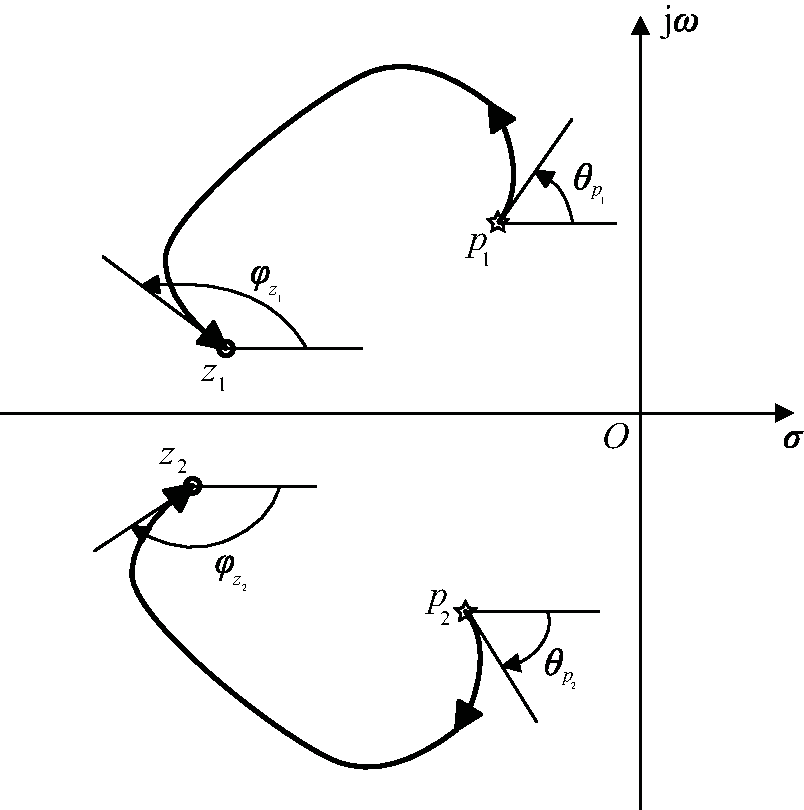
\includegraphics[width=0.4\linewidth]{pic/起始角和终止角.pdf}
			\caption{起始角和终止角的定义}
		\end{figure}
		\item 起始角\\
		在极点$p_i$临近处选择实验点$s$,若$s$位于根轨迹上,则
		\begin{align*}
			& \quad \,\,\, \sum_{j = 1}^{m}\angle (s - z_j) - \sum_{i = 1}^{n} \angle(s - p_i) = 180 \degree (2k + 1)\\
			&\Rightarrow 	\sum_{j = 1}^{m}\angle (s - z_j) - \sum_{k = 1, k \neq i }^{n} \angle(s - p_k)  - \angle (s - p_i) = 180 \degree (2k + 1) \\
			&\Rightarrow \angle (s - p_i) = 180 \degree (2k + 1) + \sum_{j = 1}^{m}\angle (s - z_j) - \sum_{k = 1, k \neq i }^{n} (s - p_k) 
		\end{align*}
		所以
	\begin{align}
		\theta_{p_i} = \lim\limits_{s \to p_i} \angle (s - p_i) =  180 \degree (2k + 1) + \sum_{j = 1}^{m}\angle (p_i - z_j) - \sum_{k = 1, k \neq i }^{n} (p_i - p_k) 
	\end{align}
	\vspace*{-1em}
	\begin{figure}[!htb]
		\begin{center}
			\begin{minipage}{0.45\linewidth}
				\centering
				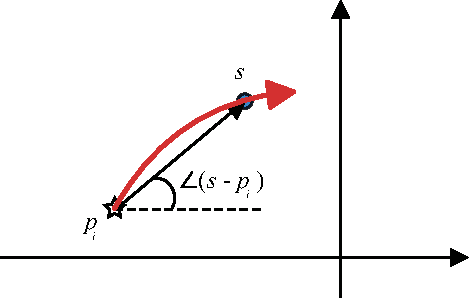
\includegraphics[width=0.9\linewidth]{pic/起始点.pdf}
				\caption{起始角的计算}
			\end{minipage}
			\begin{minipage}{0.45\linewidth}
				\centering
				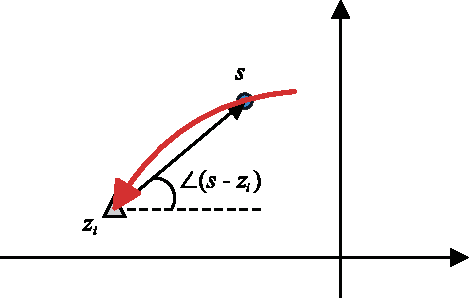
\includegraphics[width=0.9\linewidth]{pic/终止点.pdf}
				\caption{终止角的计算}
			\end{minipage}
		\end{center}
	\end{figure}
	\vspace*{-1em}
	\item 终止角\\
	在零点$z_i$临近处选择实验点$s$,若$s$位于根轨迹上,则
	\begin{align*}
		& \quad \,\,\, \sum_{j = 1}^{m}\angle (s - z_j) - \sum_{i = 1}^{n} \angle(s - p_i) = 180 \degree (2k + 1)\\
		&\Rightarrow 	\sum_{j = 1, j \neq i}^{m}\angle (s - z_j) + \angle (s - z_i)- \sum_{k = 1}^{n} \angle(s - p_k) = 180 \degree (2k + 1) \\
		&\Rightarrow \angle (s - z_i) = 180 \degree (2k + 1) + \sum_{k = 1}^{n} \angle(s - p_k) - \sum_{j = 1, j \neq i}^{m}\angle (s - z_j)
	\end{align*}
	所以
	\begin{align}
		\theta_{p_i} = \lim\limits_{s \to z_i} \angle (s - p_i) =  180 \degree (2k + 1) + \sum_{k = 1}^{n} \angle(z_i - p_k) - \sum_{j = 1, j \neq i}^{m}\angle (z_i - z_j)
	\end{align}
	\end{itemize}


	\item \textbf{根轨迹与虚轴的交点}
	\vspace*{-1em}
	\begin{itemize}
		\item 方法一 \quad 交点上的$K^*$值和$\omega$值可以用劳斯判据进行计算
		\item 方法二 \quad 令闭环特征方程中的$s = \text{j}\omega$,然后分别令其实部和虚部为零求得,即
		\begin{align}
			D(s) = \left[\prod_{i = 1}^n (s - p_i) + K^* \prod_{j = 1}^{m}(s - z_j) \right]_{s=\text{j}\omega} = 0 \quad \Longleftrightarrow \quad 
			\begin{cases}
				\text{Re}\left[D(s)\right] = 0\\
				\text{Im}\left[D(s)\right] = 0
			\end{cases}
		\end{align}
	\end{itemize}

	
	\item \textbf{根之和与根之积}\\
	令
	\begin{align*}
		G(s)H(s) = K^* \dfrac{\displaystyle \prod_{j = 1}^m (s - z_j)}{\displaystyle \prod_{i = 1}^n (s - p_i)}
	\end{align*}
	则系统闭环特征多项式为
	\begin{align*}
		&\quad \prod_{i = 1}^n (s - p_i) + K^*\prod_{j = 1}^m (s - z_j) = \prod_{i = 1}^n(s - s_i)\\
		& = s^n + a_1 s^{n-1} + \cdots + a_{n-1}s + a_n
	\end{align*}
	其中,
	\begin{align}
		a_1 = - \sum_{i = 1}^n s_i, \quad \quad a_n = (-1)^n \prod_{i=1}^{n} s_i 
	\end{align}
\begin{itemize}
	\item 闭环特征根的负值之和等于闭环特征方程第二项系数$a_1$。若$n - m \ge 2$,根之和与开环根轨迹增益$K^*$无关,即根之和不变。
	\item 闭环特征根之积乘以$(-1)^n$等于闭环特征方程的常数项。	
\end{itemize}
	
\end{enumerate}

\subsection{极点零点对消问题}
若$G(s)$的极点与$H(s)$的零点相同,将产生零极点对消,使系统的阶数降低。在绘制这种系统的根轨迹时,若使用9个基本法则,那么需要保留被消去的极点和零点进行计算分析。

\examples \label{例题4}考虑如图\ref{例题4系统结构图}所示系统:

\begin{figure}[!htb]
	\centering
	\begin{tikzpicture}[circuit ee IEC,node distance=1.2cm]
		\node[bulb] (A) [draw, inner sep = 5pt, label=-85:$-$]{};
		\node[bulb] (B) [draw, right of = A, node distance = 1.5cm,inner sep = 5pt, label=-85:$-$]{};
		\node (C) [draw, inner sep =6pt, right of = B,node distance =2cm]{$\dfrac{K^*}{(s + 1)(s + 3)}$};
		\node (D) [draw, inner sep =6pt, right of = C,node distance = 2.5cm]{$\dfrac{1}{s}$};
		
		\draw[arrows={-Stealth}] (-1cm,0cm) -- (A)node[near start, above = 0cm]{$r(t)$};
		\draw[arrows={-Stealth}] (A) -- (B)node[midway, above = 0cm]{$e(t)$};
		\draw[arrows={-Stealth}] (B) -- (C);
		\draw[arrows={-Stealth}] (C) -- (D);
		\draw[arrows={-Stealth}] (D) -- +(1.5cm,0cm)node[near end,above = 0cm]{$c(t)$};
		\draw[arrows={-Stealth}] (5cm, 0cm) --+(0cm,-1.6cm) --+ (-3.5cm,-1.6cm) -- (B);
		\draw[arrows={-Stealth}] (6.75cm, 0cm) -- +(0cm,-2.5cm) -- (0cm, -2.5cm) -- (A);
	\end{tikzpicture}
	\caption{\ref{例题4}系统结构图}
	\label{例题4系统结构图}
\end{figure}

其可等效成如图\ref{例题4系统结构等效图}所示的系统。

\begin{figure}[!htb]
	\centering
	\begin{tikzpicture}[circuit ee IEC,node distance=1.2cm]
	\node[bulb] (A) [draw, inner sep = 5pt, label=-85:$-$]{};
	\node (C) [draw, inner sep =6pt, right of = B,node distance =2cm]{$\dfrac{K^*}{(s + 1)(s + 3)}$};
	\node (D) [draw, inner sep =6pt, right of = C,node distance = 2.5cm]{$\dfrac{1}{s}$};
	\node (E) [draw, inner sep =6pt, below of = C, node distance = 2.5cm]{$(s + 1)$};
	
	\draw[arrows={-Stealth}] (-1cm,0cm) -- (A)node[near start, above = 0cm]{$r(t)$};
	\draw[arrows={-Stealth}] (A) -- (C)node[near start, above = 0cm]{$e(t)$};
	\draw[arrows={-Stealth}] (C) -- (D);
	\draw[arrows={-Stealth}] (D) -- +(1.5cm,0cm)node[near end,above = 0cm]{$c(t)$};
	\draw[arrows={-Stealth}] (6.75cm, 0cm) -- +(0cm,-2.5cm) --(E);
	\draw[arrows={-Stealth}] (E) -- (0cm, -2.5cm) -- (A);
	\end{tikzpicture}
	\caption{\ref{例题4}系统结构等效图}
	\label{例题4系统结构等效图}
\end{figure}

因此,可得
\begin{align*}
	G(s)H(s) = \dfrac{K^*(s + 1)}{s(s+1)(s+3)}
\end{align*}
其零点和极点分布为
\begin{align*}
	\begin{cases}
		\,\, p_1 = 0, \,\, p_2 = -1, \,\, p_3 = -3\\
		\,\, z_1 = -1
	\end{cases}
\end{align*}

由法则4,由于区间$[-3,0]$右侧总有奇数个极点和零点之和,因此实轴上只有区间$[-3,0]$上存在根轨迹。

由法则6,根轨迹的分离点满足
\begin{align*}
	\dfrac{1}{d - z_1} = \dfrac{1}{d - p_1} + \dfrac{1}{d - p_2} + \dfrac{1}{d - p_3}
\end{align*}
即
\begin{align*}
	\dfrac{1}{d +1} = \dfrac{1}{d} + \dfrac{1}{d + 1} + \dfrac{1}{d + 3} \quad \Rightarrow \quad 
	d + d + 3 = 0 \quad \Rightarrow \quad d = -1.5
\end{align*}
所以根轨迹的分离汇合点为$d = -1.5$

由法则5,渐近线与实轴的交角
\begin{align*}
	\varphi_a = \dfrac{(2k + 1)}{3 - 1} \times 180\degree =180\degree\times \dfrac{2k + 1}{2} = 
	\begin{cases}
		\,\, 90\degree, &k = 0\\
		\,\, -90 \degree, & k = -1
	\end{cases} 
\end{align*}
渐近线与实轴的交点
\begin{align*}
	\sigma_a = \dfrac{p_1 + p_2 + p_3 - z_1}{n - m} = \dfrac{0 -1 - 3 +1}{3 - 1} = -1.5
\end{align*}

所以,正确的根轨迹概略图如图\ref{例题4根轨迹图}.
\begin{figure}[!htb]
	\centering
	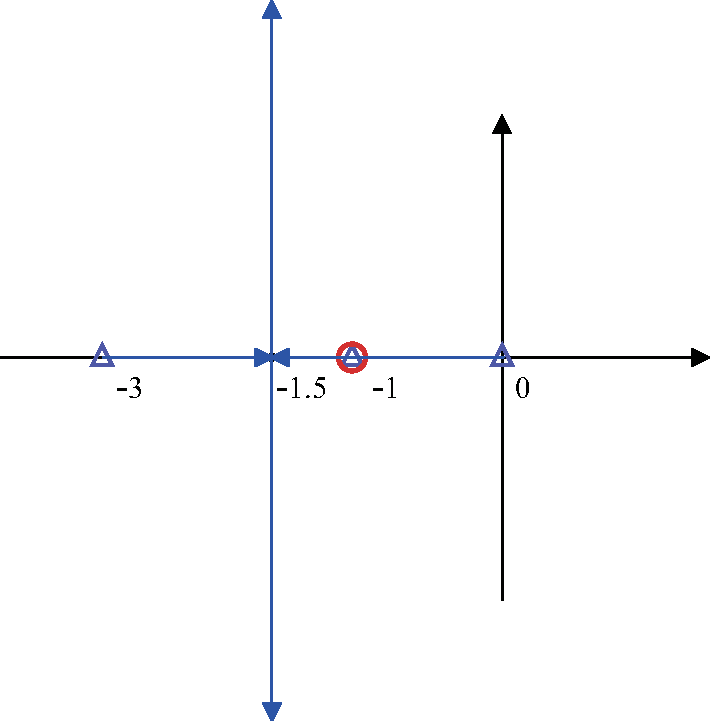
\includegraphics[width=0.45\linewidth]{pic/例题4图.pdf}
	\caption{\ref{例题4}根轨迹图}
	\label{例题4根轨迹图}
\end{figure}




\section{广义根轨迹}
在上一节我们讨论的是开环增益变化的情况,对于其他量变化的情况,单独分离出变化量即可。
\vspace*{0.5em}

\subsection{开环极点变化时的根轨迹}
\vspace*{-1em}

\examples  \label{例题4-2}已知系统的开环函数为
\begin{align}
	G(s)H(s) = \dfrac{K}{s(s+1)(T_a s + 1)}
\end{align}
尝试绘制当开环增益$K$为$0.5,1,2$时,时间常数$T_a : 0 \to \infty$时的根轨迹。
\newpage
\vspace*{-2.5em}
\solve 
\begin{itemize}
	\item 系统特征方程为
	\begin{align*}
		D(s)  = s(s+1)(T_as +1) + K = 0
	\end{align*}
	\item 将与$T_a$相关的项与其他项分离
	\begin{align*}
		D(s) = \big[s(s+1)+K\big] + s(s+1)T_a = 0
	\end{align*}
	\item 写出等效传递函数
	\begin{align*}
		G_1(s)H_1(s) = \dfrac{T_as^2(s+1)}{s^2 + s +K}
	\end{align*}
	\item 当$K$分别取$0.5,1,2$时,分别得到具体的\dy[等效传递函数]{DXCDHS}\footnote{等效传递函数是指两个系统具有相同的闭环特征方程,但具有不同的闭环传递函数,即闭环极点相同,而零点不一定相同。},求出零点和极点后,利用基本的9个法则绘制概略的根轨迹图即可。这个题的结果如图\ref{例题4-2根轨迹图}.
\end{itemize}
\begin{figure}[!htb]
	\centering
	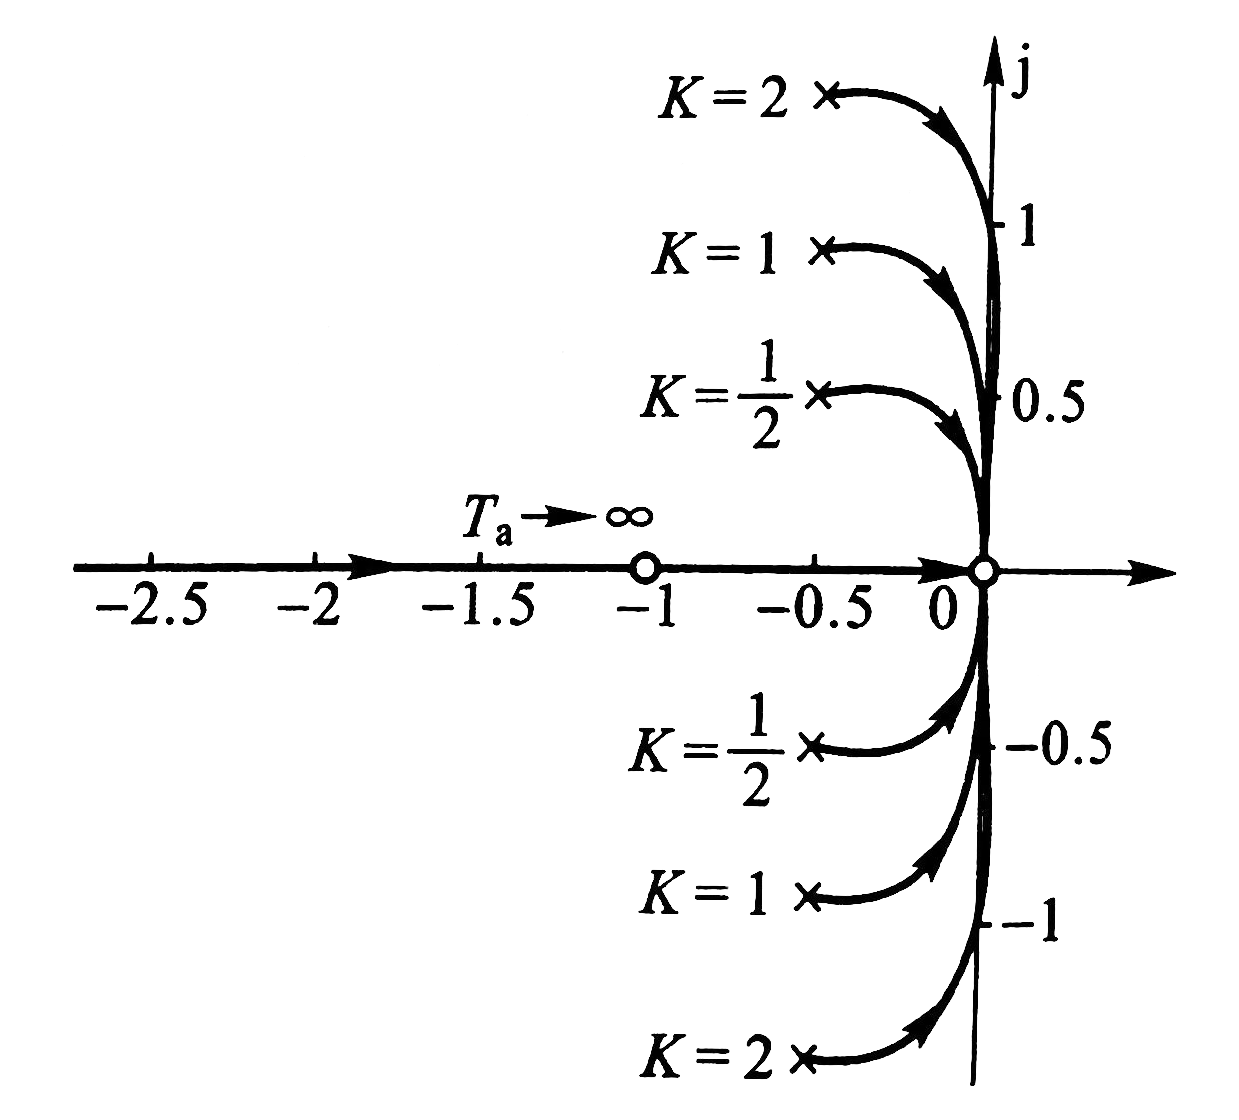
\includegraphics[width=0.45\linewidth]{pic/例题4-2.png}
	\caption{\ref{例题4-2}根轨迹图}
	\label{例题4-2根轨迹图}
\end{figure}

\subsection{零度根轨迹}
某些复杂控制系统,如飞控系统,其内回路中有正反馈,如图所示。为了分析控制系统的性能,有时需要求出内回路的闭环零、极点。

考虑典型正反馈闭环系统
\begin{figure}[!htb]
	\centering
	\begin{tikzpicture}[circuit ee IEC]
		\node(A) [draw, inner sep =6pt]{$G(s)$};
		\node(B) [draw, inner sep =6pt, below of = A, node distance = 1cm]{$H(s)$};
		\node[bulb] (O) [draw, inner sep =5pt, left of = A, node distance = 2cm, label = -95:$+$]{};
		
		\draw[arrows={-Stealth}](-3cm, 0) -- (O)node[near start, above = 0mm]{$R(s)$} -- (A)node[midway, above = 0mm]{$E(s)$} -- (2cm, 0cm)node[midway, above = 0mm,xshift = 5mm]{$C(s)$};
		\draw[arrows={-Stealth}](1.5cm, 0cm) -- +(0cm, -1cm) -- (B) -- (-2cm,-1cm) -- (O)node[midway, xshift =5mm,yshift =1mm]{$B(s)$};
	\end{tikzpicture}
	\caption{典型正反馈闭环系统}
\end{figure}

开环传递函数
\begin{align}
	G(s)H(s) = K^*\dfrac{\displaystyle \prod_{i = 1}^{m}(s - z_i)}{\displaystyle \prod_{i = 1}^{n}(s - p_i)}
\end{align}

闭环特征方程$1 - G(s)H(s) = 0$可写为
\begin{align}
	1 - K^*\dfrac{\displaystyle \prod_{i = 1}^{m}(s - z_i)}{\displaystyle \prod_{i = 1}^{n}(s - p_i)} = 0 \quad \quad \Rightarrow \quad \quad K^*\dfrac{\displaystyle \prod_{i = 1}^{m}(s - z_i)}{\displaystyle \prod_{i = 1}^{n}(s - p_i)} = 1
\end{align}
模方程和相方程分别为
\begin{align}
	K^*\dfrac{\displaystyle \prod_{i = 1}^{m}|s - z_i|}{\displaystyle \prod_{i = 1}^{n}|s - p_i|} = 1
\end{align}
\vspace*{-2em}
\begin{align}
	\textcolor{red}{\angle G(s)H(s) = \sum_{i = 1}^{m} \angle(s-z_i) - \sum_{i = 1}^n \angle(s - p_1) = 360\degree \cdot k, \quad k = 0, \pm1, \cdots}
\end{align}
与典型负反馈系统相比,模方程不变,相角相差$180\degree$.故所有与相方程有关的法则都要改,与模方程相关的法则不变。即

\begin{enumerate}[\textbf{法则} 1\hspace*{1em}]
	\item \textbf{根轨迹的分支数}
	\begin{align*}
		\mbox{分支数} &= \mbox{开环极点数}\\
		&=\mbox{开环特征方程的阶数}
	\end{align*}
	\item \textbf{根轨迹的连续性与对称性}\\
	\textbf{根轨迹是连续曲线,且对称于实轴。}
	\begin{equation*}
		\mbox{闭环极点} \,\,
		\begin{cases}
			\,\,\mbox{实数} \longrightarrow \mbox{在实轴上}\\
			\,\,\mbox{复数} \longrightarrow \mbox{共轭} \longrightarrow \mbox{对称于实轴}
		\end{cases}
	\end{equation*}
	
	\item \textbf{根轨迹的起点和终点}\\
	根轨迹起于开环极点,终于开环零点或无穷远处。\\
	
	\item \textbf{实轴上的根轨迹}\\
	实轴上某一区域,如果它右边开环实数零点、极点的个数之和为\textcolor{red}{偶数},则该区域必是根轨迹。
	
	\item \textbf{根轨迹的渐进线}\\
	若$n < m$,则有$n - m$个开环零点在无穷远处,则有$n - m$条根轨迹将沿着一组渐近线趋于无穷远点。
	\begin{itemize}
		\item 渐近线与实轴的交角
		\begin{align}
			\phi_\text{a} = \dfrac{\textcolor{red}{360 \degree} k}{n-m}, \quad k = 0,\pm 1,\pm 2, \cdots,\pm (n-m-1)
		\end{align}
		\item 渐近线与实轴的交点
		\begin{align}
			\sigma_\text{a} = \dfrac{\displaystyle \sum_{i =1}^n p_i - \sum_{j = 1}^m z_j}{n-m}
		\end{align}
	\end{itemize}
	
	\item \textbf{根轨迹的分离点(汇合点)}
		\begin{align}
			\sum_{j = 1}^{m} \dfrac{1}{d - z_j} = \sum_{i =1}^{n}\dfrac{1}{d - p_i}
		\end{align}
		分离角为$\dfrac{180 \degree}{k}$,其中$k$为汇合点处极点的个数。
	
	\item \textbf{根轨迹的起始角和终止角}
	\begin{itemize}
		\item 起始角
		\begin{align}
			\theta_{p_i} = \lim\limits_{s \to p_i} \angle (s - p_i) =  \textcolor{red}{360 \degree k}  + \sum_{j = 1}^{m}\angle (p_i - z_j) - \sum_{k = 1, k \neq i }^{n} (p_i - p_k) 
		\end{align}
		\item 终止角
		\begin{align}
			\theta_{p_i} = \lim\limits_{s \to z_i} \angle (s - p_i) =  \textcolor{red}{360 \degree k} + \sum_{k = 1}^{n} \angle(z_i - p_k) - \sum_{j = 1, j \neq i}^{m}\angle (z_i - z_j)
		\end{align}
	\end{itemize}
	
	
	\item \textbf{根轨迹与虚轴的交点}
	\vspace*{-1em}
	\begin{itemize}
		\item 方法一 \quad 交点上的$K^*$值和$\omega$值可以用劳斯判据进行计算
		\item 方法二 \quad 令闭环特征方程中的$s = \text{j}\omega$,然后分别令其实部和虚部为零求得,即
		\begin{align}
			D(s) = \left[\prod_{i = 1}^n (s - p_i) \textcolor{red}{-} K^* \prod_{j = 1}^{m}(s - z_j) \right]_{s=\text{j}\omega} = 0 \quad \Longleftrightarrow \quad 
			\begin{cases}
				\text{Re}\left[D(s)\right] = 0\\
				\text{Im}\left[D(s)\right] = 0
			\end{cases}
		\end{align}
	\end{itemize}
	
	
	\item \textbf{根之和与根之积}\\
	令
	\begin{align*}
		G(s)H(s) = K^* \dfrac{\displaystyle \prod_{j = 1}^m (s - z_j)}{\displaystyle \prod_{i = 1}^n (s - p_i)}
	\end{align*}
	则系统闭环特征多项式为
	\begin{align*}
		&\quad \prod_{i = 1}^n (s - p_i) + K^*\prod_{j = 1}^m (s - z_j) = \prod_{i = 1}^n(s - s_i)\\
		& = s^n + a_1 s^{n-1} + \cdots + a_{n-1}s + a_n
	\end{align*}
	其中,
	\begin{align}
		a_1 = - \sum_{i = 1}^n s_i, \quad \quad a_n = (-1)^n \prod_{i=1}^{n} s_i 
	\end{align}
	\begin{itemize}
		\item 闭环特征根的负值之和等于闭环特征方程第二项系数$a_1$。若$n - m \ge 2$,根之和与开环根轨迹增益$K^*$无关,即根之和不变。
		\item 闭环特征根之积乘以$(-1)^n$等于闭环特征方程的常数项。	
	\end{itemize}
	
\end{enumerate}

\vspace*{-2.5em}

\examples \label{4.3}已知正反馈系统的开环传递函数如下
\begin{align}
	G(s) = \dfrac{K^*}{s(s+1)(s+3)}
\end{align}
绘制其概略根轨迹。

\solve 其极点为
\begin{align*}
	p_1 = 0 \quad \quad p_2 = -1 \quad \quad p_3 = -3
\end{align*}

由法则4,由于区间$[-3,-1],[0,+\infty)$右侧总有偶数数个极点和零点之和,因此实轴上只有区间$[-3,-1],[0,+\infty)$上存在根轨迹。

由法则6,根轨迹的分离点满足
\begin{align*}
	\dfrac{1}{d - z_1} = \dfrac{1}{d - p_1} + \dfrac{1}{d - p_2} + \dfrac{1}{d - p_3}
\end{align*}
即
\begin{align*}
	0 = \dfrac{1}{d} + \dfrac{1}{d + 1} + \dfrac{1}{d + 3} \quad \Rightarrow \quad 
	3d^2 + 8d + 3 = 0 \quad \Rightarrow \quad d = \,
	\begin{cases}
		\, \dfrac{- \sqrt{7} - 4 }{3} \approx -2.22 \\[0.5em]
		\, \dfrac{\sqrt{7} - 4}{3} \approx  -0.45 \mbox{舍去}
	\end{cases}
\end{align*}
所以根轨迹的分离汇合点为$d = -2.22 $

由法则5,渐近线与实轴的交角
\begin{align*}
	\varphi_a = \dfrac{(k)}{3} \times 360\degree =
	\begin{cases}
		\,\, 0\degree, &k = 0\\
		\,\, 120 \degree, & k = -1\\
		\,\, -120 \degree, & k = -1
	\end{cases} 
\end{align*}
渐近线与实轴的交点
\begin{align*}
	\sigma_a = \dfrac{p_1 + p_2 + p_3}{n - m} = \dfrac{0 -1 - 3 }{3} = -\dfrac{4}{3}
\end{align*}

所以,正确的根轨迹概略图如图\ref{F4.3}.


\begin{figure}[!htb]
	\centering
	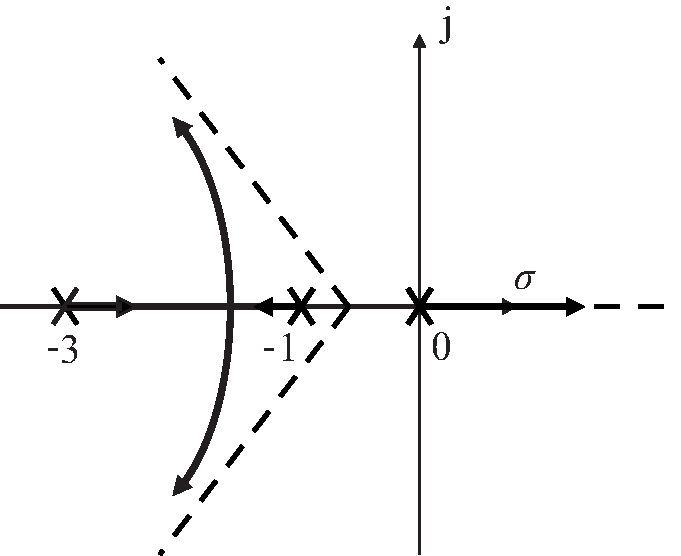
\includegraphics[width=0.3\linewidth]{pic/4.3.pdf}
	\caption{\ref{4.3}根轨迹图}
	\label{F4.3}
\end{figure}

\subsection{非最小相位系统}
若所有极点和零点均位于左半平面,称系统为\dy[最小相位]{ZXXW}的;若至少有一个零点或极点位于右半平面,则称系统为\dy[非最小相位]{FZXXW}的。

对于非最小相位的根轨迹,只需要将表达式化成标准形式
\footnote[1]{传递函数的标准形式(一二阶环节的标准形式见\pageref{一阶系统的标准形式}页):每个环节$s$的系数均大于0,且开环增益系数$K>0$,满足标准形式后若多出一个负号则为零度根轨迹,否则为一般根轨迹。}
再按照对应的系统根轨迹法则绘制即可。


\section{系统阶跃响应的根轨迹分析}

\subsection{主导极点与偶极子}
\tdefination[主导极点]
距离虚轴最近且附近没有闭环零点的一些闭环极点对系统的动态过程性能影响最大,起主要决定作用,称为\dy[主导极点]{ZDJD}。

工程上往往只用主导极点估算系统的动态性能,即将系统近似地看成一阶或二阶系统。
\vspace*{0.5em}

\defination[偶极子]
一对靠得很近的闭环零点、极点称为\dy[偶极子]{OJZ}。
\vspace*{1em}

\subsection{利用主导极点估算系统的性能指标}
既然主导极点在动态过程中起主要作用,那么,计算性能指标时,在一定条件下就可以只考虑暂态分量中主导极点对应的分量,将高阶系统近似看做一、二阶系统,直接应用第三章中计算性能指标的公式和曲线。

\examples \label{4.4}某单位负反馈系统的开环传递函数为
\begin{align*}
	G(s) = \dfrac{K}{s(s + 1)(0.5s + 1)}
\end{align*}
试应用根轨迹法分析系统的稳定性,并计算闭环主导极点具有阻尼比0.5时的性能指标。
\vspace*{1em}

\solve 
\vspace*{-2.9em}
\begin{align*}
	G(s) = \dfrac{K}{s(s + 1)(0.5s + 1)} = \dfrac{2K}{s(s + 1)(s + 2)}
\end{align*}

按步骤作出系统的根轨迹,如图\ref{F4.4}所示。

\begin{figure}[!htb]
	\centering
	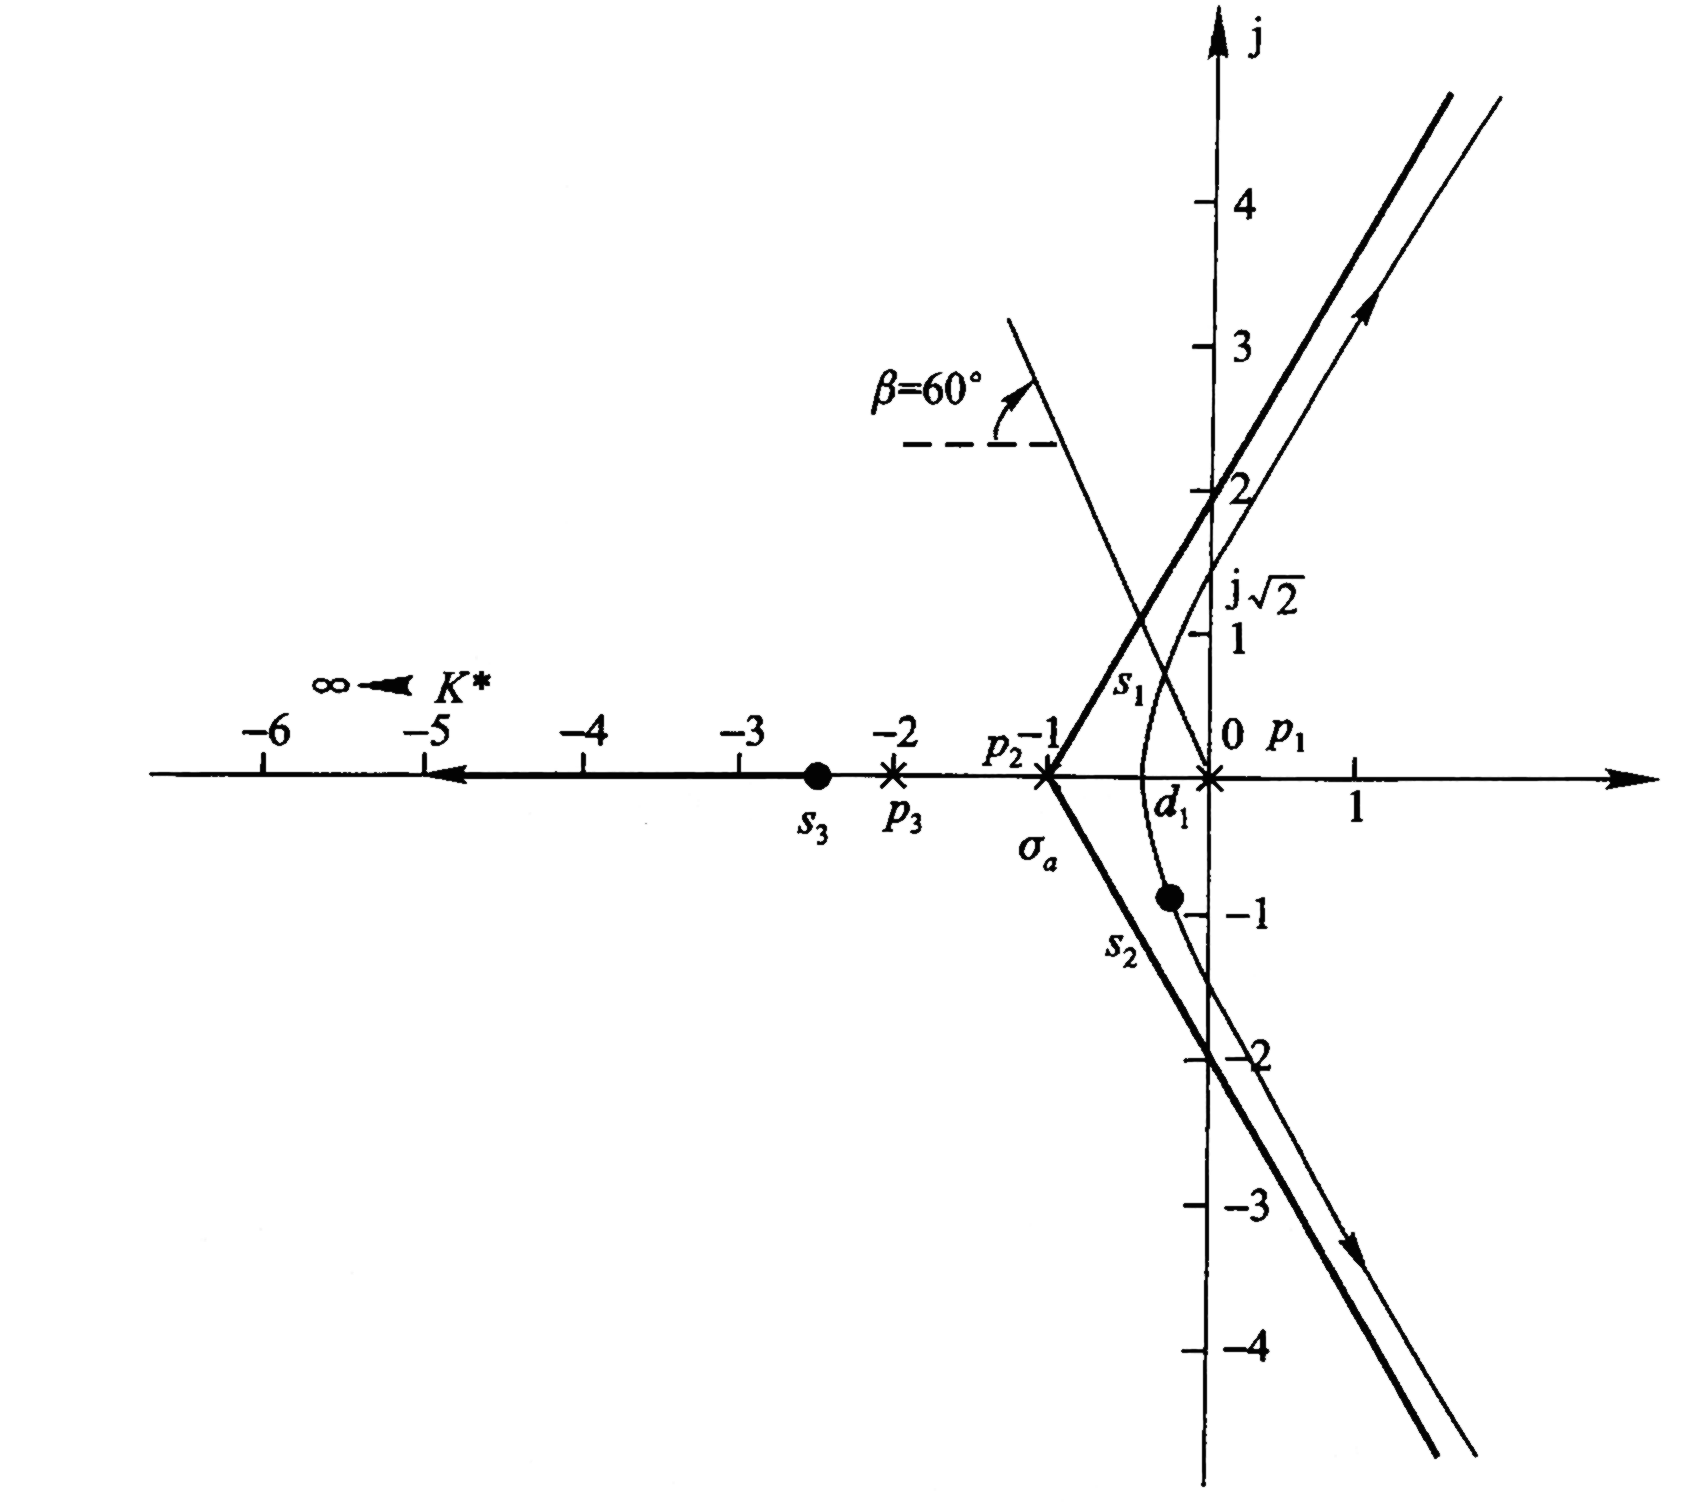
\includegraphics[width=0.62\linewidth]{pic/4.4.png}
	\vspace*{-1.2em}
	\caption{\ref{4.4}根轨迹图}
	\label{F4.4}
\end{figure}

分析系统稳定性: 系统稳定的开环增益范围是 $0<K<3$.
	
在平面上画出$\zeta =0.5$时的阻尼线,求$\zeta = 0.5$阻尼线与根轨迹交点的方法:\textcolor{red}{待定系数法}。
\begin{align*}
	D(s) &= s^3 + 3 s^2 + 2s + K^*\\
	& = \left(s^2 + 2 \zeta \omega_ns + \omega_n^2 \right)(s + s_3)\\
	& = s^3 + (2 \zeta \omega_n + s_3)s^2 +(\omega_n^2 + 2\zeta \omega_ns_3)s + s_3\omega_n^2
\end{align*}
比对系数可得
\begin{align*}
	\begin{cases}
		\, 2 \zeta \omega_n + s_3 = 3\\
		\, \omega_n^2 + 2\zeta \omega_ns_3 = 2 \\
		\, s_3\omega_n^2 = K^*
	\end{cases}
\quad \quad 
\xrightarrow{\quad \textstyle \zeta = 0.5 \quad }
\quad \quad 
	\begin{cases}
		\, \omega_n = 2/3 \approx 0.667\\
		\, s_3 = 7/3 \approx 2.333\\
		\, K^* = 28/27 \approx 1.037
	\end{cases}
\end{align*}
所以$D(s) = (s^2 + 0.667s + 0.445)(s + 2.333)$,解得特征根为
\begin{align*}
	s_{1,2} = -0.33 \pm 0.58 \j \quad \quad s_3 = -2.33
\end{align*}
由于$s_3$到虚轴到距离是$s_{1,2}$的7倍,所以$s_{1,2}$是主导极点。根据其来估算系统性能。即
\begin{align*}
	\varPhi(s) = \dfrac{1.037}{(s^2 + 0.667s + 0.445)(s + 2.333)} \approx  \dfrac{0.445}{s^2 + 0.667s + 0.445}
\end{align*}
二阶系统在单位阶跃信号作用下的性能指标为
\begin{align*}
	\sigma \% = \e ^{\zeta \pi / \sqrt{1 - \zeta^2}} &\times 100 \% = \e^{-0.5\times 3.14/\sqrt{1 - 0.5^2}} \times 100 \% = 16.3 \% \\
	t_{\text{s}} &= \dfrac{3.5}{\zeta \omega_n} = \dfrac{3.5}{0.5 \times 0.667} = 10.5 \text{s}
\end{align*}
\vspace*{1em}

\subsection{系统阶跃响应的根轨迹分析}
\vspace*{-1em}
\examples \label{4.5}已知系统结构如图\ref{F.4.5}所示。试画出当$K^*$由$0\to +\infty$时的闭环根轨迹,并分析$K^*$对系统动态过程的影响。
\begin{figure}[!htb]
	\centering
	\begin{tikzpicture}[circuit ee IEC]
		\node(A) [draw, inner sep =5pt]{$\,\,\dfrac{K^*(s+4)}{s(s+2)}\,\,$};
		\node[bulb] (O) [draw, inner sep =5pt, left of = A, node distance = 2cm, label = -95:$-$]{};
		
		\draw[arrows={-Stealth}](-3cm, 0) -- (O)node[near start, above = 0mm]{$R(s)$} -- (A) -- (2cm, 0cm)node[midway, above = 0mm,xshift = 5mm]{$C(s)$};
		\draw[arrows={-Stealth}](1.5cm, 0cm) -- +(0cm, -1cm) -- (-2cm,-1cm) -- (O);
	\end{tikzpicture}
	\caption{\ref{4.5} 系统结构图}
	\label{F.4.5}
\end{figure}

\solve 利用根轨迹的法则,可以画出这个带零点的二阶系统的根轨迹,其复数部分为一个圆,其圆心在开环零点处,半径为零点到分离点的距离。
\begin{figure}[!htb]
	\centering
	
\includegraphics[width=0.5\linewidth]{pic/4.5.png}
	\caption{\ref{4.5} 系统根轨迹图}
	\label{F.4.5.1}
\end{figure}
根轨迹分离点为
\begin{align*}
	d_1 = -1.172, \quad d_2 = -6.83
\end{align*}
由模方程,对应开环增益
\begin{align*}
	K_1^* = \dfrac{|d_1||d_1 + 2|}{|d_1 + 4|} = \dfrac{1.172 \times 0.828}{2.828} = 0.343 \quad \quad K_1 = 2K_1^*=0.686\\[0.5em]
	K_2^* = \dfrac{|d_2||d_2 + 2|}{|d_2 + 4|} = \dfrac{6.83 \times 4.83}{2.83} = 11.7 \quad \quad K_2 = 2K_2^*=23.4
\end{align*}

根轨迹如图\ref{F.4.5.1}所示:
\begin{itemize}
	\item $0<K<0.686$\\
	闭环为两个负实数极点,系统在阶跃信号下响应为非周期的。
	\item $0.686<K<23.4$\\
	闭环为一对共轭复数极点,其阶跃响应为振荡衰减过程。
	\item $K>23.4$\\
	闭环又为负实数极点,其阶跃响应非周期的。
	
	\item 特别地,系统最佳阻尼比对应的极点\\
	过原点作与根轨迹圆相切的直线,与负实轴夹角的余弦即为系统的阻尼比
	\begin{align*}
		\zeta = \cos \beta = \cos 45\degree = 0.707
	\end{align*}
	对应闭环极点
	\begin{align*}
		s_{1,2} = - 2 \pm \j 2
	\end{align*}
	此时系统阶跃响应具有较好的平稳性。
\end{itemize}
\warn[
{
	\begin{minipage}{0.6\linewidth}
		\textbf{二阶系统阻尼比在根轨迹上的表示}\\
		\hspace*{2em}对于标准形式的二阶系统,其特征方程及对应特征根为
		\begin{align*}
			s^2 + 2 \zeta \omega_{\text{n}} s + \omega_{\n}^2 &= 0
		\end{align*}
		\vspace*{-3em}
		\begin{align*}
			s_{1,2} &= - \zeta \omega_{\n} \pm \omega_{\n}\sqrt{\zeta^2 - 1} \quad (\zeta \le 1)\\
			&= - \zeta \omega_{\n} \pm \j \, \omega_{\n}\sqrt{1 - \zeta^2} \quad (0 <\zeta < 1)
		\end{align*}

		如图\ref{阻尼比在根轨迹上的表示}所示,则
		\begin{align*}
			\cos \beta = \dfrac{\zeta}{\sqrt{\zeta^2 + (1 - \zeta^2)}} = \zeta
		\end{align*}
	\end{minipage}
	\begin{minipage}{0.4\linewidth}
		\centering
		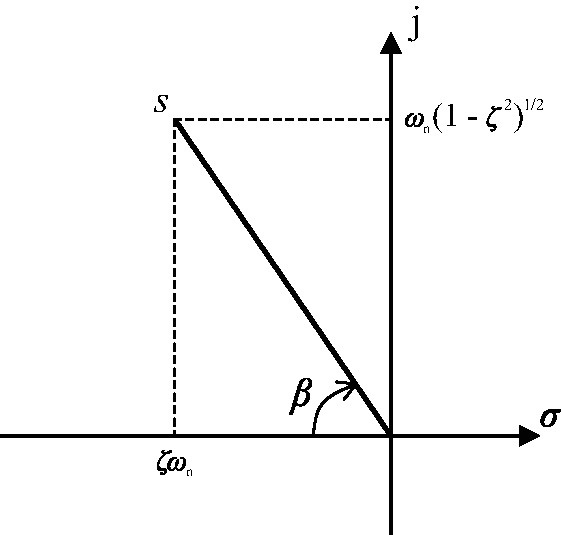
\includegraphics[width=0.8\linewidth]{pic/阻尼比的表示.pdf}
		\captionof{figure}{阻尼比在根轨迹上的表示}
		\label{阻尼比在根轨迹上的表示}
	\end{minipage}
}
]

\subsection{系统闭环根轨迹的改造}
\vspace*{-1em}
\examples \label{4.6}单位反馈系统的开环传递函数
\begin{align*}
	G(s) = \dfrac{K^*}{s^2(s+10)}
\end{align*}
按步骤作出系统的根轨迹,如图\ref{F4.6.1}所示。显然,系统结构不稳定。此时,通过增加零点改善系统动态性能,并利用根轨迹进行分析。
\begin{figure}[!htb]
	\centering
	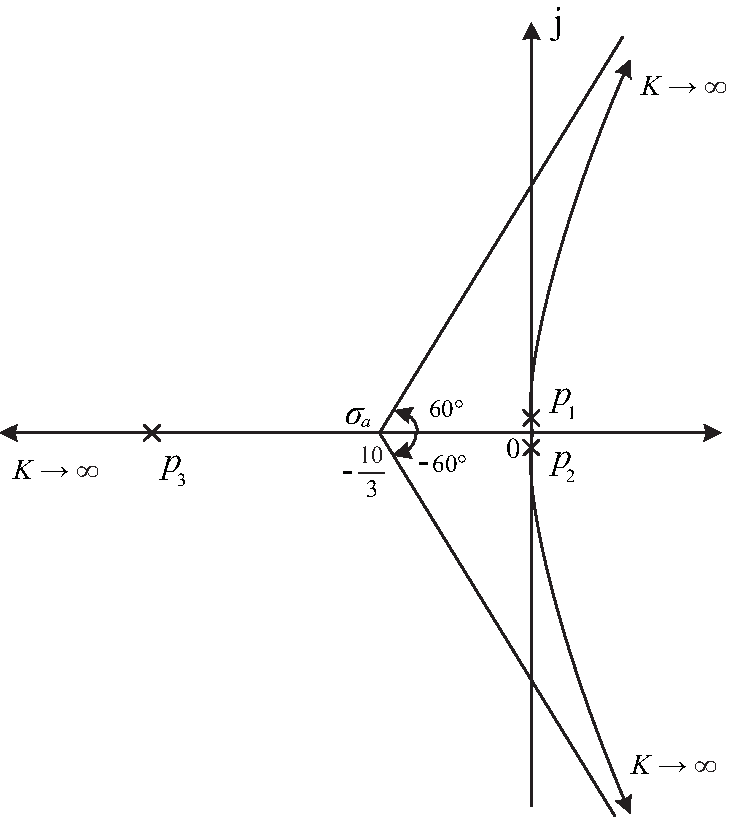
\includegraphics[width=0.4\linewidth]{pic/4.6.1.pdf}
	\caption{\ref{4.6}根轨迹图}
	\label{F4.6.1}
\end{figure}

增加零点$z_1$后的开环传递函数为
\begin{align*}
	G(s) = \dfrac{K^*(s - z_1)}{s^2(s+10)}
\end{align*}

\begin{figure}[!htb]
\begin{minipage}{0.5\linewidth}

		\centering
		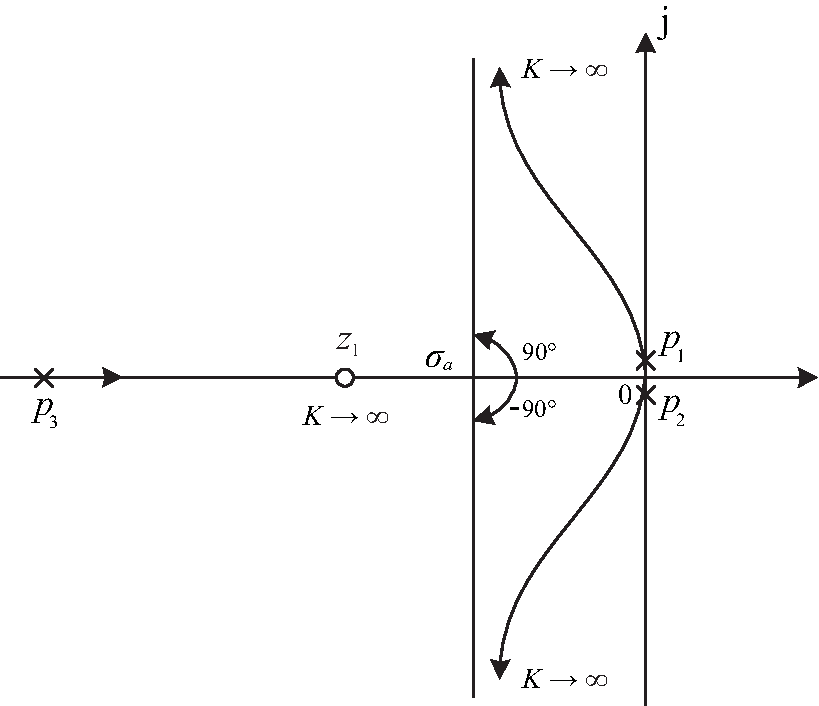
\includegraphics[width=0.98\linewidth]{pic/4.6.2.pdf}
		\caption{\ref{4.6}改进根轨迹图1}
		\label{F4.6.2}
\end{minipage}
\begin{minipage}{0.5\linewidth}
		\centering
		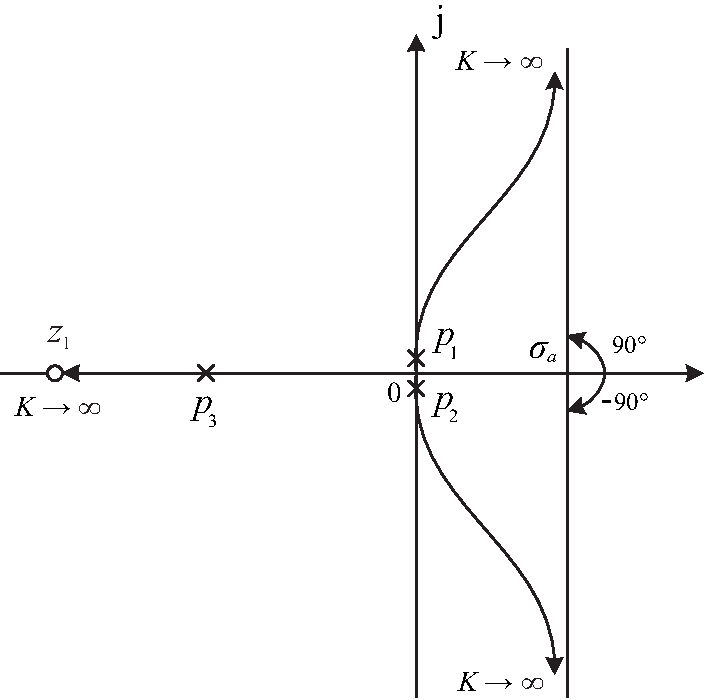
\includegraphics[width=0.85\linewidth]{pic/4.6.3.pdf}
		\caption{\ref{4.6}改进根轨迹图2}
		\label{F4.6.3}
\end{minipage}
\end{figure}
\begin{itemize}
	\item $ 0 < z_1 < 10$\\
	系统的根轨迹如图\ref{F4.6.2}所示。可见,系统稳定,但总有一对共轭复极点。系统单位阶跃响应振荡衰减且振荡频率随K的增大而增大。
	
	\item $z_1 < -10$\\
	系统的根轨迹如图\ref{F4.6.3}所示,系统总是不稳定的。因此,引入零点要恰当才能改善系统的性能。
\end{itemize}

\section{利用Matlab绘制根轨迹}
	此部分暂时省略。













